\documentclass[conference]{IEEEtran}
\IEEEoverridecommandlockouts

\usepackage{cite}
\usepackage{amsmath,amssymb}
\usepackage{graphicx}
\usepackage{booktabs}
\usepackage{multirow}
\usepackage{xcolor}
\usepackage{tikz}
\usetikzlibrary{arrows.meta,positioning,fit,backgrounds,calc}
\usepackage{pgfplots}
\pgfplotsset{compat=1.17}
\usepackage[hidelinks]{hyperref}
\usepackage{url}

\definecolor{ssblue}{RGB}{31,119,180}
\definecolor{ssorange}{RGB}{230,85,13}
\definecolor{ssgreen}{RGB}{44,160,44}
\definecolor{ssgrey}{RGB}{110,110,110}
\definecolor{sspurple}{RGB}{117,107,177}

\newcommand{\Lmax}{L_{\max}}
\newcommand{\Cl}{C_{\mathrm{L}}}
\newcommand{\Cr}{C_{\mathrm{R}}}

\begin{document}

\title{Character Recall Is Not Protection: A Document-Level Leakage Analysis of Bounded-Memory PII and Credential Redaction for Operational Logs}

\author{
\IEEEauthorblockN{Mounish Senisetty\IEEEauthorrefmark{1}, Sandhiya Kennedy, Ashrith Reddy N, Parvathy R}
\IEEEauthorblockA{Amrita School of Computing, Amrita Vishwa Vidyapeetham, Amritapuri, Kerala, India\\
\IEEEauthorrefmark{1}am.ai.u4aid23058@am.students.amrita.edu, am.ai.u4aid23056@am.students.amrita.edu,\\
am.ai.u4aid23014@am.students.amrita.edu, parvathyr@am.amrita.edu}
}

\maketitle

\begin{abstract}
Automated redaction of personal data and credentials is routinely judged by
character- or entity-level recall, yet a shared log file is safe only if
\emph{every} sensitive span in it is removed. We study this gap for
redactors that must also run in bounded memory over multi-gigabyte logs. We
first describe a boundary-safe streaming redactor whose window overlap is
derived from per-detector locality bounds, so that chunked and multi-worker
execution cannot cut a detection in half at a buffer seam. We then propose a
leakage-centric evaluation protocol that classifies every ground-truth span as
fully redacted, partially redacted or missed, and reports the document
no-leak rate, a leak-tolerance curve, leak concentration and shape-stratified
leak rates, together with an oracle union-of-systems ceiling. Applying the
protocol to five redaction systems on 8{,}002 mandatory spans in 95 held-out
documents shows that the best single configuration fully redacts 80.5\% of
spans yet leaves 82.1\% of documents leaking; even the union of all five
systems misses 8.2\% of spans and leaves 72.6\% of documents exposed.
Passwords embedded in prose leak at 87--97\% for every system. The redactor
holds net resident memory between 8.4 and 8.54\,MiB from 8\,MiB to 2\,GiB of
input and scales to 41.1\,MB/s on four workers. The results argue for
reporting document-level leakage alongside recall and against using any
current automatic redactor as an unsupervised release gate.
\end{abstract}

\begin{IEEEkeywords}
data redaction, personally identifiable information, secret detection, data leakage, streaming algorithms, evaluation methodology
\end{IEEEkeywords}

%=====================================================================
\section{Introduction}
%=====================================================================

Application logs, database exports and incident captures are copied between
teams, vendors and analytics platforms every day. They routinely carry
personally identifiable information (PII), such as e-mail addresses, phone
numbers and payment cards, alongside credentials such as API keys, bearer
tokens and private keys. Credentials in particular continue to leak at scale
through software artefacts~\cite{meli2019git,krause2023pushed}, and
organisational data-loss-prevention controls~\cite{manmadhan2014dlp} rarely
inspect the content of bulk text before it leaves a team.

Automatic redaction tools fall into two largely separate families: PII
de-identification frameworks such as Microsoft Presidio~\cite{presidio}, and
secret scanners such as gitleaks~\cite{gitleaks} and
TruffleHog~\cite{trufflehog}. Both are usually evaluated with precision and
recall at character or entity level. For a person deciding whether a file may
be shared, however, the relevant question is binary: \emph{did anything
sensitive survive?} A redactor that masks 95\% of sensitive characters can
still leak something in nearly every document if the remaining 5\% is spread
thinly. Recall averages hide exactly this failure mode.

A second, engineering-level obstacle appears when the input is large. A
multi-gigabyte log cannot be redacted as one in-memory string, so it is read
in chunks. A secret that straddles a chunk boundary is then seen only in
fragments, and neither fragment may match a detector. Ad-hoc overlaps reduce
but do not remove this boundary leak.

This paper addresses both problems and makes the following contributions:
\begin{enumerate}
\item \textbf{Boundary-safe bounded-memory redaction.} We describe a streaming
and multi-worker redactor in which every detector declares upper bounds on the
span length it emits and the context it reads; the engine derives the minimum
window overlap from these bounds, defers detections that cross the emission
cut, and cross-checks worker seams with a sequential fallback
(Section~\ref{sec:system}).
\item \textbf{A leakage-centric evaluation protocol.} Beyond character
metrics, we classify every ground-truth span as fully redacted, partially
redacted or missed, and report the document no-leak rate, a $k$-leak tolerance
curve, leak concentration, shape-stratified leak rates and an oracle
union-of-systems ceiling (Section~\ref{sec:protocol}).
\item \textbf{An empirical leakage study.} We compare five redaction
configurations from three tool families on three held-out corpora and show
that document-level protection is far below what recall suggests, that
combining every tool does not close the gap, and that passwords in prose are a
shared blind spot (Section~\ref{sec:results}).
\end{enumerate}

%=====================================================================
\section{Related Work}
%=====================================================================

\textit{De-identification of text.} Text de-identification began in clinical
informatics with dictionary and pattern systems~\cite{neamatullah2008deid},
later refined by Philter~\cite{norgeot2020philter}, shared-task
corpora~\cite{stubbs2015annotating} and recurrent sequence
labellers~\cite{dernoncourt2017deid}. Presidio~\cite{presidio} combines
pattern recognisers with spaCy or transformer models, and generalist
span-extraction models such as GLiNER~\cite{zaratiana2024gliner} broaden entity
coverage. Lison \emph{et al.}~\cite{lison2021anonymisation} argue that masking
surface entities is not the same as anonymisation, and the Text Anonymization
Benchmark~\cite{pilan2022tab} introduced document-level and re-identification
oriented metrics for legal text. Our protocol follows the same spirit but
targets mixed PII and credential leakage in operational text, and adds span
outcome classes and a cross-system ceiling.

\textit{Credential detection.} Secret detection moved from vendor regular
expressions~\cite{sinha2015secretkey} to learned false-positive
filters~\cite{saha2020secrets} and password classifiers~\cite{feng2022passfinder}.
SecretBench~\cite{basak2023secretbench} standardised evaluation, and a
nine-tool comparison~\cite{basak2023comparative} traced low precision to broad
patterns and uncalibrated entropy thresholds. Named-entity models have also
been adapted to security text~\cite{simran2020cyberner}. These tools target
version-controlled source trees; their behaviour on free-form logs and prose
is rarely measured.

\textit{Streaming text processing.} Sublinear-memory processing of unbounded
inputs is studied in the data-stream model~\cite{muthukrishnan2005streams},
and security pipelines already score continuous message streams, for example
for threat indicators~\cite{simran2020twitter}. Such pipelines score short,
self-contained messages and do not face entities split across buffers. In the
redaction tools we surveyed, window overlaps are chosen by hand, and no
analytical lower bound on the overlap is stated.

%=====================================================================
\section{Boundary-Safe Streaming Redaction}
\label{sec:system}
%=====================================================================

\begin{figure}[t]
\centering
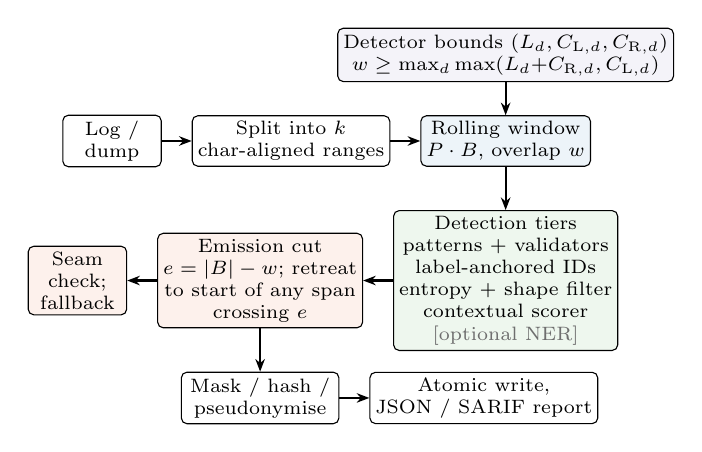
\begin{tikzpicture}[
  font=\scriptsize,
  box/.style={draw, rounded corners=2pt, align=center, minimum height=0.62cm, inner sep=2pt, fill=white},
  arr/.style={-{Stealth[length=1.6mm]}, thick},
  grp/.style={draw, dashed, rounded corners=3pt, inner sep=4pt}
]
\node[box, minimum width=1.25cm] (in) {Log /\\ dump};
\node[box, right=0.38cm of in, minimum width=2.0cm] (split) {Split into $k$\\ char-aligned ranges};
\node[box, right=0.38cm of split, minimum width=2.05cm, fill=ssblue!8] (win) {Rolling window\\ $P\cdot B$, overlap $w$};

\node[box, below=0.55cm of win, minimum width=2.05cm, fill=ssgreen!8] (det) {Detection tiers\\ patterns + validators\\ label-anchored IDs\\ entropy + shape filter\\ contextual scorer\\ {\color{ssgrey}[optional NER]}};
\node[box, left=0.38cm of det, minimum width=2.0cm, fill=ssorange!8] (cut) {Emission cut\\ $e=|B|-w$; retreat\\ to start of any span\\ crossing $e$};
\node[box, left=0.38cm of cut, minimum width=1.25cm, fill=ssorange!8] (seam) {Seam\\ check;\\ fallback};
\node[box, below=0.55cm of cut, minimum width=2.0cm] (pol) {Mask / hash /\\ pseudonymise};
\node[box, right=0.38cm of pol, minimum width=2.05cm] (out) {Atomic write,\\ JSON / SARIF report};

\node[box, above=0.42cm of win, minimum width=2.05cm, fill=sspurple!8] (decl) {Detector bounds $(L_d,C_{\mathrm{L},d},C_{\mathrm{R},d})$\\ $w\ge\max_d\max(L_d{+}C_{\mathrm{R},d},C_{\mathrm{L},d})$};

\draw[arr] (in) -- (split);
\draw[arr] (split) -- (win);
\draw[arr] (win) -- (det);
\draw[arr] (det) -- (cut);
\draw[arr] (cut) -- (seam);
\draw[arr] (cut) -- (pol);
\draw[arr] (pol) -- (out);
\draw[arr] (decl) -- (win);
\end{tikzpicture}
\caption{Redaction pipeline. Detectors declare locality bounds from which the
engine derives the window overlap $w$; detections crossing the emission cut
are deferred to the next pass, and parallel seams are cross-checked before
output is assembled.}
\label{fig:arch}
\end{figure}

Fig.~\ref{fig:arch} summarises the reference redactor used in this study. It is
a local tool with a pure-Python reference implementation and an optional Rust
core for the pattern and entropy tiers; no plaintext is sent to any network
service.

\subsection{Detection Tiers}
\textit{Patterns with validators} match fixed-format credentials (cloud access
keys, vendor API tokens, JSON web tokens, PEM private keys) and structured PII
(e-mail, phone, payment card, US SSN, IPv4/IPv6). A candidate survives only if
its validator accepts it: Luhn checksums~\cite{luhn1960} for cards, range rules
for SSNs, octet and hextet ranges for IP literals and E.164 structure for
phone numbers. \textit{Label-anchored identifiers} emit bare numeric record,
account or licence numbers only when a domain anchor such as ``Patient ID:''
occurs within the preceding 96 characters. \textit{The entropy tier} scores
unstructured tokens of 20--8192 characters by Shannon entropy~\cite{shannon1948},
character-class diversity and length, and a \emph{benign-shape filter}
suppresses 40- or 64-hex digests preceded by hash-like labels and inline
\texttt{data:} URIs unless an assignment to a secret-like key precedes them.
A \textit{contextual scorer} adjusts confidence from a 48-character left
context. An optional spaCy NER tier extracts names, organisations and places;
it lies outside the boundary guarantee below because its receptive field is
not statically bounded.

\subsection{Overlap Derivation and Emission Retreat}
Each detector $d$ declares an upper bound $L_d$ on the length of any span it
emits and bounds $C_{\mathrm{L},d}$ and $C_{\mathrm{R},d}$ on the left and
right context its decision may read. The streaming engine keeps a context
buffer $P$ of the last $w$ emitted characters and a look-ahead buffer $B$. Each
pass runs the detectors on $P\cdot B$, keeps detections that start inside $B$,
and nominally emits up to the cut $e=|B|-w$. If a kept detection $(i,j)$
satisfies $i<e<j$, the cut retreats to $i$, so the span is emitted whole in a
later pass. If
\begin{equation}
w \;\ge\; \max_d \max\!\left(L_d + C_{\mathrm{R},d},\; C_{\mathrm{L},d}\right),
\label{eq:overlap}
\end{equation}
every detection emitted in a pass has its full declared context inside the
window, and every detection crossing the cut is seen again intact in the next
window. The streamed span set therefore equals the whole-document span set for
any chunking, which removes boundary leaks for all detectors that honour their
declared bounds. The engine computes (\ref{eq:overlap}) at start-up and rejects
any smaller user-supplied overlap. For the shipped deterministic tiers the
largest constants are $C_{\mathrm{L}}=96$, $C_{\mathrm{R}}=8$ and
$L_{\max}=8192$, and the 8192-character spans come from detectors that read no
right context, so the default overlap is $w=8192$.

\subsection{Parallel Seams}
For large files the byte stream is split into $k$ ranges aligned to UTF-8 code
points, each processed by a separate worker with $w$ characters of read-only
context on either side. A detection crossing an interior seam belongs to the
left worker; the right worker starts emitting at the end of that detection.
Both neighbours compute the hand-off offset independently from their own view
of the seam, and the coordinator compares them before assembling output. Any
disagreement triggers a sequential re-run, so parallel output is byte-identical
to sequential output or falls back to it. Working memory is bounded by
$O(k(w+m+c))$ characters for minimum emit size $m$ and chunk size $c$,
independent of input length.

\subsection{Verification}
An automated suite of 133 tests checks byte-for-byte identity between
whole-document, streamed and multi-worker execution under exhaustive
small-step chunkings, property-based random inputs, entities planted across
seams and injected seam disagreements that must trigger the fallback, as well
as Rust--Python parity and the declared detector bounds. On all three test
splits the two backends produced identical span sets.

%=====================================================================
\section{Leakage-Centric Evaluation Protocol}
\label{sec:protocol}
%=====================================================================

Let $G_d$ be the set of ground-truth sensitive spans in document $d$ and $R_d$
the set of characters a system masks. Entity labels are ignored throughout: a
span counts as protected if its characters are masked, whatever class the
system assigned.

\textit{Character metrics.} Character precision $|G\cap R|/|R|$ and recall
$|G\cap R|/|G|$ are macro-averaged over documents, and F1 is their harmonic
mean. They are reported for comparability with prior work.

\textit{Span outcome classes.} Each span $s\in G_d$ is \emph{fully redacted}
if all its characters are in $R_d$, \emph{partially redacted} if some but not
all are, and \emph{missed} otherwise. Partial redaction is counted as a leak,
because a partially exposed card number or key can permit brute force or
record linkage~\cite{sweeney2002kanonymity}. The fully redacted rate (FR) is
the share of spans in the first class.

\textit{Document no-leak rate.} A document is \emph{leak-free} if every
mandatory span is fully redacted. The no-leak rate is the fraction of
documents that are leak-free; it is the metric a release gate would need.

\textit{$k$-leak tolerance curve.} Because the no-leak rate is strict, we also
report the fraction of documents with at most $k$ leaked spans for
$k\in\{0,1,2,5,10\}$. The curve shows whether failures are near misses that a
human reviewer could fix quickly or pervasive.

\textit{Leak concentration and composition.} We report the median length of
leaked spans, the share of leaked characters that come from partial rather
than missed spans, and the share of all leaked characters that fall in the
10\% of documents that leak most.

\textit{Shape-stratified leak rate.} When the corpus carries only sensitivity
labels, not types, we bucket gold spans by a coarse surface shape (numeric,
alphanumeric token, capitalised words, other single token, tokens containing
``@'', multi-word phrases) and report the leak rate per bucket.

\textit{Oracle union ceiling.} We take, per document, the union of characters
masked by all evaluated systems. Its leakage is an optimistic ceiling on what
any ensemble of these tools can achieve without new detectors.

\textit{False alarms and uncertainty.} On documents with no gold spans, the
false-alarm rate (FA) is the fraction with at least one emitted span.
Interval estimates use a percentile bootstrap over documents with 2{,}000
resamples~\cite{efron1994bootstrap}, and paired differences share resample
indices. For no-leak rates we also give Wilson score
intervals~\cite{wilson1927}.

%=====================================================================
\section{Experimental Setup}
%=====================================================================

\begin{table}[t]
\centering
\caption{Held-out test splits. Gold: annotated sensitive spans; gold-free:
documents with no sensitive span.}
\label{tab:corpora}
\setlength{\tabcolsep}{4pt}
\begin{tabular}{lrrrr}
\toprule
Corpus & Docs & Gold & Gold-free & Bytes \\
\midrule
presidio-research~\cite{presidioresearch} & 750 & 1{,}394 & 63 & 63{,}678 \\
secrets (Nosey Parker~\cite{noseyparker}) & 313 & 293 & 97 & 46{,}595 \\
RedactionBench~\cite{redactionbench} & 100 & 25{,}592 & 0 & 1{,}378{,}267 \\
\bottomrule
\end{tabular}
\end{table}

\textit{Corpora.} Table~\ref{tab:corpora} lists the test splits. Each corpus
was split once into development and test parts with a fixed seed, and
manifests with SHA-256 digests lock the assignment. \emph{presidio-research}
is the synthetic benchmark shipped with Presidio's evaluation suite.
\emph{secrets} contains credential examples from the Nosey Parker rule
catalogue, split by rule so that test vendors are unseen, plus 200 synthetic
gold-free documents of UUIDs, Git hashes, SHA-256 digests, base64 images and
minified JavaScript. \emph{RedactionBench} contains multi-paragraph documents
in eleven domains with character-level \emph{mandatory} and \emph{contextual}
labels; 95 of its 100 test documents contain at least one mandatory span, for
8{,}002 mandatory spans with a median of 25 per document. All RedactionBench
documents were inspected during error analysis before the split, so we also
report a pre-exposure code revision.

\textit{Systems.} \emph{SafeStream} (the redactor of
Section~\ref{sec:system}) runs on the Rust core in its deterministic
configuration (\emph{pattern}) and with the spaCy \texttt{en\_core\_web\_sm}
tier (\emph{+spaCy}). \emph{Presidio} 2.2.355~\cite{presidio} runs with
patterns only (\emph{regex}) and with the \texttt{en\_core\_web\_sm}
(\emph{sm}) and \texttt{en\_core\_web\_lg} (\emph{lg}) models.
\emph{gitleaks} 8.28.0 and \emph{TruffleHog} 3.90.8 run with their default
rules; TruffleHog uses \texttt{--no-verification} so that no candidate
credential is sent to a live endpoint. The two scanners are designed for Git
repositories and are evaluated here out of their native domain, which is the
setting in which practitioners often repurpose them for log sanitisation.

\textit{Environment.} Accuracy and throughput were measured on a Linux virtual
machine with a 4-vCPU Intel Xeon (2.80\,GHz), 15\,GB RAM and CPython 3.13.
Python baselines ran single-threaded; throughput figures are means of five
trials on an otherwise idle host.

%=====================================================================
\section{Results}
\label{sec:results}
%=====================================================================

\subsection{Character Metrics Overstate Protection}

\begin{table}[t]
\centering
\caption{Held-out character F1, fully redacted rate (FR) and false-alarm
document rate (FA), with 95\% bootstrap intervals for F1. +spaCy rows lie
outside the boundary guarantee.}
\label{tab:summary}
\setlength{\tabcolsep}{3.2pt}
\begin{tabular}{llccc}
\toprule
Corpus & System & Char F1 & FR & FA \\
\midrule
\multirow{4}{*}{\shortstack[l]{presidio-\\research}}
 & SafeStream pattern & .267 [.235,.299] & .115 & .000 \\
 & SafeStream +spaCy  & .702 [.679,.725] & .538 & .079 \\
 & Presidio regex     & .296 [.260,.333] & .123 & .000 \\
 & Presidio lg        & .665 [.642,.688] & .562 & .000 \\
\midrule
\multirow{4}{*}{secrets}
 & SafeStream pattern & .842 [.736,.906] & .437 & .010 \\
 & gitleaks           & .604 [.430,.765] & .311 & .000 \\
 & TruffleHog         & .306 [.204,.446] & .270 & .000 \\
 & Presidio lg        & .184 [.124,.262] & .164 & .433 \\
\bottomrule
\end{tabular}
\end{table}

Table~\ref{tab:summary} gives the conventional view. On \emph{secrets} the
deterministic tiers reach character F1 of 0.842 and a fully redacted rate of
0.437, against 0.311 for gitleaks and 0.270 for TruffleHog; the paired
bootstrap differences in FR, +0.128 [+0.073,\,+0.183] and +0.167
[+0.079,\,+0.250], exclude zero. Presidio has no credential recognisers and
raises a false alarm on 43.3\% of gold-free documents. On
\emph{presidio-research}, pattern-only systems cap at F1 below 0.30 because
most gold spans are unstructured names and places; adding a statistical NER
tier lifts F1 to about 0.7 for both SafeStream and Presidio.

On RedactionBench the final SafeStream configurations reach mandatory
character recall of 0.682 (pattern) and 0.761 (+spaCy), against 0.420 for
Presidio lg, 0.247 for gitleaks and 0.024 for TruffleHog. The document no-leak
rates tell a different story: 8 of 95 documents (8.4\%, Wilson 95\% interval
[4.3,\,15.7]\%) for SafeStream pattern, 17 (17.9\% [11.5,\,26.8]) for
SafeStream +spaCy, 10 (10.5\% [5.8,\,18.3]) for Presidio lg, 2 for gitleaks and
none for TruffleHog. A configuration that masks three quarters of mandatory
characters thus produces a fully clean document fewer than one time in five.

\subsection{Anatomy of Leaks}

\begin{table}[t]
\centering
\caption{Outcome of the 8{,}002 mandatory spans in RedactionBench test
documents. Partial: share of leaked characters from partially redacted spans.
Top-10\%: share of leaked characters in the 10\% most-leaking documents.}
\label{tab:outcomes}
\setlength{\tabcolsep}{2.6pt}
\begin{tabular}{lrrrrrr}
\toprule
System & Full & Part. & Missed & \shortstack{Leaked\\chars} & \shortstack{Partial\\share} & \shortstack{Top-\\10\%} \\
\midrule
SafeStream pattern & 5{,}688 & 68  & 2{,}246 & 22{,}778 & 3.7\%  & 59.3\% \\
SafeStream +spaCy  & 6{,}441 & 64  & 1{,}497 & 17{,}122 & 4.8\%  & 66.8\% \\
Presidio lg        & 5{,}614 & 395 & 1{,}993 & 41{,}589 & 17.7\% & 53.7\% \\
gitleaks           & 232     & 0   & 7{,}770 & 53{,}991 & 0.0\%  & 61.0\% \\
TruffleHog         & 43      & 1   & 7{,}958 & 69{,}913 & 0.0\%  & 53.0\% \\
\midrule
Union of all five  & 7{,}048 & 295 & 659     & 9{,}214  & 32.2\% & 70.1\% \\
\bottomrule
\end{tabular}
\end{table}

Table~\ref{tab:outcomes} decomposes the leaks. Three observations stand out.

\emph{Leaks are mostly whole misses, not boundary errors.} For both SafeStream
configurations fewer than 1\% of spans are partially redacted and partial
spans contribute under 5\% of leaked characters. Presidio lg produces about
six times as many partial spans (395 against 64) and draws 17.7\% of its
leaked characters from them, consistent with NER span boundaries that disagree
with annotation boundaries. Partial redaction matters because the exposed
remainder of a structured value may be enough to reconstruct it.

\emph{Leaked spans are short and word-like.} The median leaked span is 7
characters for SafeStream pattern and 9 for +spaCy and Presidio lg: the length
of a name, a short identifier or a password. Such spans fall below the
20-character minimum of the entropy tier and lack the fixed structure that
pattern tiers rely on, so they escape detectors built for keys and tokens.

\emph{Leakage is concentrated.} The 10\% of documents that leak most hold
53--70\% of all leaked characters. Median leaked spans per document are 11 for
SafeStream pattern, 6 for +spaCy and 8 for Presidio lg, while the worst
document leaks at least 313 spans for every system.

\begin{figure}[t]
\centering
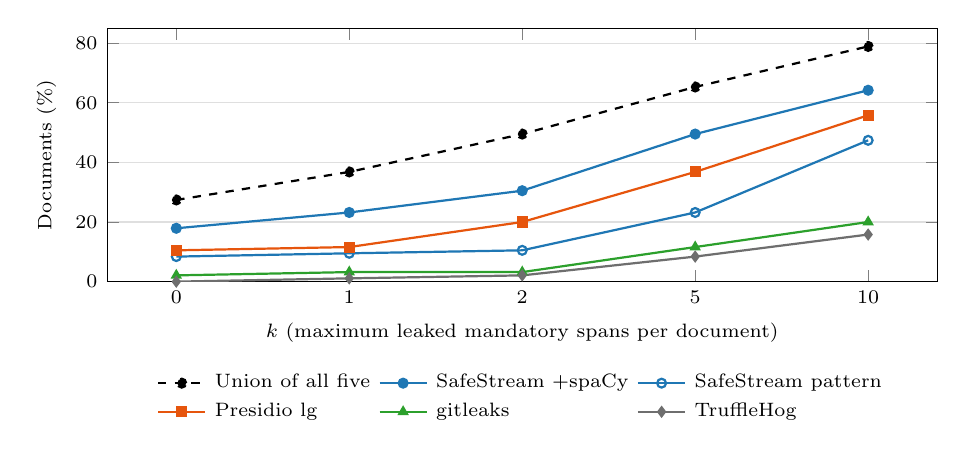
\begin{tikzpicture}
\begin{axis}[
  width=\columnwidth, height=4.8cm,
  symbolic x coords={0,1,2,5,10},
  xtick=data,
  xlabel={$k$ (maximum leaked mandatory spans per document)},
  ylabel={Documents (\%)},
  ymin=0, ymax=85,
  ymajorgrids, grid style={gray!25},
  legend style={font=\scriptsize, at={(0.5,-0.32)}, anchor=north, draw=none, legend columns=3, column sep=1pt, cells={anchor=west}},
  tick label style={font=\scriptsize}, label style={font=\scriptsize},
  every axis plot/.append style={thick, mark size=1.6pt}
]
\addplot[color=black, mark=*, dashed] coordinates {(0,27.4) (1,36.8) (2,49.5) (5,65.3) (10,78.9)};
\addplot[color=ssblue, mark=*] coordinates {(0,17.9) (1,23.2) (2,30.5) (5,49.5) (10,64.2)};
\addplot[color=ssblue, mark=o] coordinates {(0,8.4) (1,9.5) (2,10.5) (5,23.2) (10,47.4)};
\addplot[color=ssorange, mark=square*] coordinates {(0,10.5) (1,11.6) (2,20.0) (5,36.8) (10,55.8)};
\addplot[color=ssgreen, mark=triangle*] coordinates {(0,2.1) (1,3.2) (2,3.2) (5,11.6) (10,20.0)};
\addplot[color=ssgrey, mark=diamond*] coordinates {(0,0.0) (1,1.1) (2,2.1) (5,8.4) (10,15.8)};
\legend{Union of all five, SafeStream +spaCy, SafeStream pattern, Presidio lg, gitleaks, TruffleHog}
\end{axis}
\end{tikzpicture}
\caption{$k$-leak tolerance curve on the 95 RedactionBench test documents
with mandatory spans. $k=0$ is the no-leak rate.}
\label{fig:tolerance}
\end{figure}

Fig.~\ref{fig:tolerance} shows the $k$-leak tolerance curve. Allowing up to
two leaked spans per document raises SafeStream +spaCy from 17.9\% to 30.5\%
of documents; allowing ten raises it to 64.2\%. Even at $k=10$ more than a
third of documents still leak more than ten mandatory spans, so the residual
is not a handful of near misses that a reviewer could patch in seconds.

\subsection{What Leaks: Shape-Stratified Rates}

\begin{table}[t]
\centering
\caption{Leak rate (missed or partially redacted) of RedactionBench mandatory
spans by coarse surface shape. The corpus has no type labels; shapes come from
a regular-expression heuristic.}
\label{tab:shapes}
\setlength{\tabcolsep}{3.0pt}
\begin{tabular}{lrcccc}
\toprule
Shape & Spans & \shortstack{SS\\pattern} & \shortstack{SS\\+spaCy} & \shortstack{Presidio\\lg} & Union \\
\midrule
Numeric (digits, punct.) & 4{,}604 & .137 & .130 & .114 & .048 \\
Alphanumeric token       & 1{,}619 & .187 & .177 & .716 & .143 \\
Capitalised word(s)      & 1{,}044 & .899 & .267 & .265 & .136 \\
Other single token       & 689     & .576 & .521 & .556 & .469 \\
Contains ``@''           & 38      & .974 & .947 & .921 & .868 \\
Multi-word phrase        & 8       & 1.00 & .500 & .750 & .375 \\
\bottomrule
\end{tabular}
\end{table}

Table~\ref{tab:shapes} shows where each tool family fails. Numeric spans make
up 57.5\% of mandatory spans and are handled comparably by all three PII-aware
configurations (11--14\% leak). The families diverge elsewhere. Pattern-only
SafeStream leaks 89.9\% of capitalised names, which the NER tier reduces to
26.7\%. Presidio lg leaks 71.6\% of alphanumeric tokens such as identifiers and
keys, against 18.7\% for SafeStream, reflecting the latter's credential and
label-anchored tiers. The 38 spans containing ``@'' leak at 87--97\% for every
system and even for the union; since the e-mail recognisers of SafeStream and
Presidio would catch addresses, these are predominantly passwords written in
prose. Free-text passwords have no fixed
format, often fall below entropy thresholds, and are a blind spot shared by
every tool family we evaluated.

\subsection{The Union Ceiling}

Masking the union of all five systems' outputs fully redacts 88.1\% of
mandatory spans and leaves 659 missed, 56\% fewer than the best single system.
Yet only 26 of 95 documents (27.4\%, Wilson [19.4,\,37.1]\%) become leak-free.
The union also has the highest partial share (32.2\% of leaked characters),
since overlapping detections with different boundaries cover the core of a
span but not its edges. Ensembling the tools in use today is therefore not a
route to document-level safety; the remaining leaks require new detectors,
chiefly for passwords and context-dependent identifiers.

\subsection{Contamination and False Alarms}

Because RedactionBench was inspected before splitting, the figures above are
optimistic. At the last code revision before the benchmark was added, mandatory
recall was 0.589 (pattern) and 0.674 (+spaCy) and the no-leak rates were 7.4\%
and 13.7\%. Rules written after inspection raised pattern mandatory recall by
+0.091 [+0.044,\,+0.163]; this is an upper bound on what transfers to unseen
data. On point estimates, even the pre-exposure configurations exceed every
Presidio configuration in mandatory recall (best 0.420).

High-entropy benign strings are the main false-alarm source for credential
redaction. Before the benign-shape filter was added, the entropy tier flagged
83 of the 103 gold-free documents in the secrets development split (0.806),
including every synthetic UUID, Git hash, SHA-256 digest and base64 data URI.
With the filter, the test-split false-alarm rate fell from 0.794
[0.714,\,0.872] to 0.010 [0.000,\,0.035] and character precision rose from
0.589 to 0.857, while recall (0.829) and FR (0.437) were unchanged. The test
split had been evaluated once before the filter was designed and the negatives
come from the same five-category generator, so this shows suppression of those
formats rather than of arbitrary production strings.

\subsection{Resource Cost of Bounded-Memory Operation}

\begin{figure}[t]
\centering
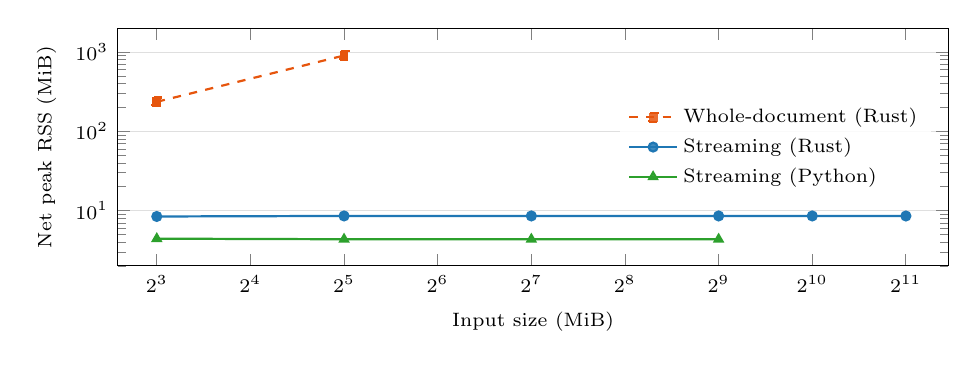
\begin{tikzpicture}
\begin{loglogaxis}[
  width=\columnwidth, height=4.6cm,
  log basis x=2,
  xlabel={Input size (MiB)}, ylabel={Net peak RSS (MiB)},
  xmin=6, xmax=2800, ymin=2, ymax=2000,
  ymajorgrids, grid style={gray!25},
  legend style={font=\scriptsize, at={(0.98,0.5)}, anchor=east, draw=none, fill=white, fill opacity=0.85, text opacity=1, cells={anchor=west}},
  tick label style={font=\scriptsize}, label style={font=\scriptsize},
  every axis plot/.append style={thick, mark size=1.6pt}
]
\addplot[color=ssorange, mark=square*, dashed] coordinates {(8,235.48) (32,904.57)};
\addplot[color=ssblue, mark=*] coordinates {(8,8.41) (32,8.54) (128,8.54) (512,8.54) (1024,8.54) (2048,8.53)};
\addplot[color=ssgreen, mark=triangle*] coordinates {(8,4.41) (32,4.34) (128,4.34) (512,4.34)};
\legend{Whole-document (Rust), Streaming (Rust), Streaming (Python)}
\end{loglogaxis}
\end{tikzpicture}
\caption{Net resident memory (peak minus post-import baseline) against input
size for a synthetic log dense with PII and credentials, one process per
point. A whole-document run on 128\,MiB did not finish within 20 minutes.}
\label{fig:memory}
\end{figure}

Fig.~\ref{fig:memory} confirms that streaming memory is flat: on the Rust core
net peak RSS stayed between 8.4 and 8.54\,MiB as input grew 256-fold from
8\,MiB to 2\,GiB, and the pure-Python backend stayed between 4.3 and 4.4\,MiB
up to 512\,MiB. Whole-document execution needed 904.6\,MiB for a 32\,MiB
input, about 28 times the input size, because the input string, match objects
and output buffer coexist.

On RedactionBench (13.8\,kB average document) the Rust core sustained
$10.4\pm1.3$\,MB/s single-threaded, against $0.069$\,MB/s for Presidio regex.
Enabling statistical NER slowed SafeStream by more than two orders of
magnitude, to 0.047\,MB/s, and Presidio sm and lg ran at 0.020\,MB/s.
On a 256\,MB log, one, two and four workers reached $10.5\pm0.5$,
$20.6\pm0.5$ and $41.1\pm1.4$\,MB/s, a $3.9\times$ speed-up with output
byte-identical to the sequential run.

%=====================================================================
\section{Discussion}
%=====================================================================

\textit{Report document-level leakage.} The gap between 76.1\% mandatory
recall and a 17.9\% no-leak rate arises because recall is an average over
characters while the no-leak rate is a conjunction over spans. With a median
of 25 mandatory spans per document, even a high per-span success rate
compounds into frequent document failure. Redaction papers and tool
evaluations should report the no-leak rate and a tolerance curve next to
recall; otherwise improvements that matter to recall but not to release safety
are indistinguishable from those that do.

\textit{Deployment implications.} No evaluated tool, nor their union, is fit to
release documents to untrusted parties without review. Two uses remain
well supported. First, as a pre-processor for human review: masking three
quarters of mandatory characters at 10\,MB/s per core reduces reviewer effort,
and boundary-safe chunking guarantees that splitting a file adds no new
artefacts. Second, as defence in depth inside access-controlled stores, where
removing most plaintext credentials from multi-gigabyte logs in fixed memory
lowers exposure without risking memory exhaustion. A two-stage layout is
natural: deterministic tiers inline on bulk telemetry, where their boundary
guarantee holds, and the slower NER tier on free-text fields such as tickets
and e-mail bodies.

\textit{Threats to validity.} presidio-research and the secrets corpus are
synthetic, and secret ground truth follows Nosey Parker capture groups.
RedactionBench was inspected before splitting (mitigated by the pre-exposure
revision) and its creators report low agreement on contextual spans, which is
why we use mandatory spans only. Document-level resampling ignores clustering
by rule and domain, so intervals may be too narrow. The shape buckets are a
heuristic, not type labels. gitleaks and TruffleHog were run outside their
repository setting and without live verification, so their results reflect
domain mismatch as well as detector coverage. All measurements were taken on
one machine with English input.

%=====================================================================
\section{Conclusion}
%=====================================================================

We presented a bounded-memory redactor whose window overlap is derived from
declared detector locality bounds, eliminating boundary leaks in streamed and
multi-worker execution, and a leakage-centric protocol for judging redactors
by whether documents come out clean. On held-out data the redactor fully
redacts 80.5\% of mandatory spans and runs in under 9\,MiB of working memory up
to 2\,GiB of input, but fewer than one document in five is leak-free, and the
union of five tools reaches only 27.4\%. Short context-dependent identifiers
and free-text passwords dominate what remains. Future work will evaluate on
real continuous-integration logs under a responsible-disclosure protocol,
develop detectors for in-prose passwords, and seek formal context bounds for
windowed neural taggers so that NER tiers can share the boundary guarantee.

\section*{Acknowledgment}
The authors thank the maintainers of Presidio, Nosey Parker and RedactionBench
for releasing their software and data. The large language model Claude
(Anthropic) was used to help write evaluation scripts and to edit the
manuscript; the authors verified all code, results and text and take full
responsibility for the content.

\bibliographystyle{IEEEtran}
\bibliography{refs}

\end{document}
